\chapter{Scenario Series 6-5}

This appendix presents simulation results from the 6-5 scenario series, this tests impact of varying tightness of even flow constraints for hardwood and softwood AAC. 

\section{Summary}
Table \ref{tab:scenario_list} below lists the scenarios in this series. 

This scenario series tests impact of varying slack in of species-wise even-flow constraints in the principal's wood supply model. 
The default slack for all other scenario series is 5\% (i.e., periodic harvest volume must be within interval $(0.95 v_{max}, 1.00 v_{max})$, where $v_{max}$ represents the maximum periodic harvest volume for a given solution). 

Increasing even-flow constraint slack seems to have a moderate negative impact on stability of harvest levels and profit. This is not entirely surprising, if one considers that the principal's wood supply plans are optimal solutions to deterministic problems, and that adding slack to the even-flow constraint produces more and more jagged (deterministic) harvest profiles. Any deviation, however small, from the optimal solution will either produce an alternative optimal solution (unlikely), a suboptimal feasible solution, or an infeasible solution. We know there are deviations in the base case (with 5\% slack), and we know this causes some measurable drift over time. Adding more variability to the optimal solutions is not likely to reduce these deviations on average.

Also, the even-flow constraints are defined \emph{species-wise}, which means that softwood harvest level might jump up in the first period while hardwood harvest jumps down. In this example, the agent would have to include a greater-than-usual proportion of pure softwood stands in his harvest plan to satisfy softwood demand while harvesting an unusually-low hardwood volume. This would tend to aggravate the existing high-grading problem, which is responsible for residual drift.

Overall, the best scenario in this series (in terms of stability, harvest level, and profit) is scenario 6-5\_hw000sw000 (i.e., perfectly tight even-flow constraints).

\begin{table}
  \centering
  \begin{tabular}{lll}
    \hline
    Scenario ID & Figure Reference & Description \\
    \hline
    3-1 & \ref{fig:s3-1} & Control (\emph{status quo}). \\
    6-5\_hw005sw005 & \ref{fig:s6-5_hw005sw005} & Hardwood: 0\%, softwood: 0\%. \\
    6-5\_hw005sw005 & \ref{fig:s6-5_hw005sw005} & Hardwood: 1\%, softwood: 1\%. \\
    6-5\_hw005sw005 & \ref{fig:s6-5_hw005sw005} & Hardwood: 5\%, softwood: 5\%. \\
    6-4\_hw099sw005 & \ref{fig:s6-5_hw099sw005} & Hardwood: 99\%, softwood: 5\%. \\
    6-4\_hw010sw010 & \ref{fig:s6-5_hw010sw010} & Hardwood: 10\%, softwood: 10\%. \\
    6-4\_hw020sw020 & \ref{fig:s6-5_hw020sw020} & Hardwood: 20\%, softwood: 20\%. \\
    6-4\_hw050sw050 & \ref{fig:s6-5_hw050sw050} & Hardwood: 50\%, softwood: 50\%. \\

    \hline
  \end{tabular}
  \caption{Description of scenarios in series 6-5.}
  \label{tab:scenario_list}
\end{table}

\section{Results}

Figures \ref{fig:s6-5_hw005sw005} to \ref{fig:s6-5_hw050sw050} present
simulation results for fifteen scenarios. % Table \ref{tab:scenarios}
% summarizes scenario parameters used in the experiment for each
% scenario.
Disposition of figures is identical for all scenarios. The
first subfigure (a) for each scenario shows the initial
(ie. iteration-0) AAC solution. The second subfigure (b) for each
scenario shows first period of AAC solution for all 30 planning
iterations. The third subfigure (c) for each scenario shows the
implemented harvest level for all 30 planning iterations. Scenarios
3.1 and 3.2 also show profit in this subfigure on a secondary
axis. The fourth subfigure (d) for each scenario shows the difference
between initial and re-planned AAC. The fifth subfigure (e) for each
scenario shows the difference between re-planned AAC and harvest.  The
sixth subfigure (f) for each scenario shows the difference between
initial AAC and harvest. Softwood volume is shown with white bars,
hardwood volume with black bars, and total volume with small
circles. Profit (where applicable) is shown with the $\times$
symbol. 


\begin{figure}[h]
  \centering
  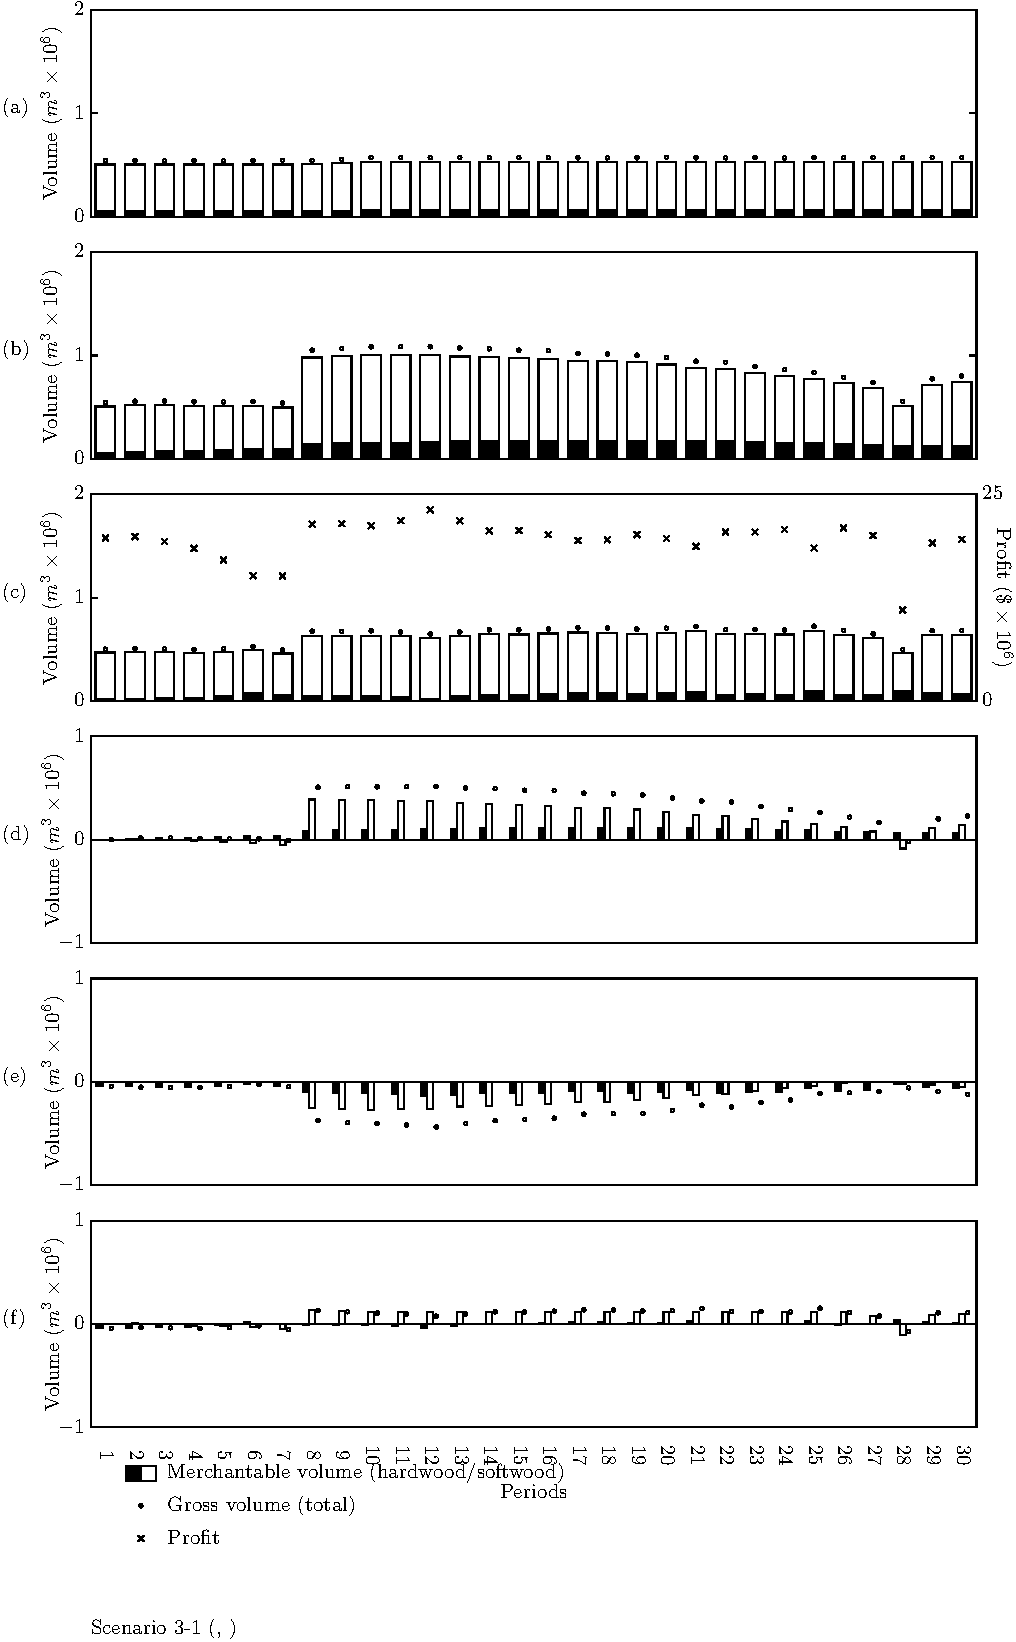
\includegraphics[width=10cm]{images/appendix/s3-1}
  \caption{Scenario 3-1 (\emph{status quo}).}
  \label{fig:s3-1}
\end{figure}

\begin{figure}[h]
  \centering
  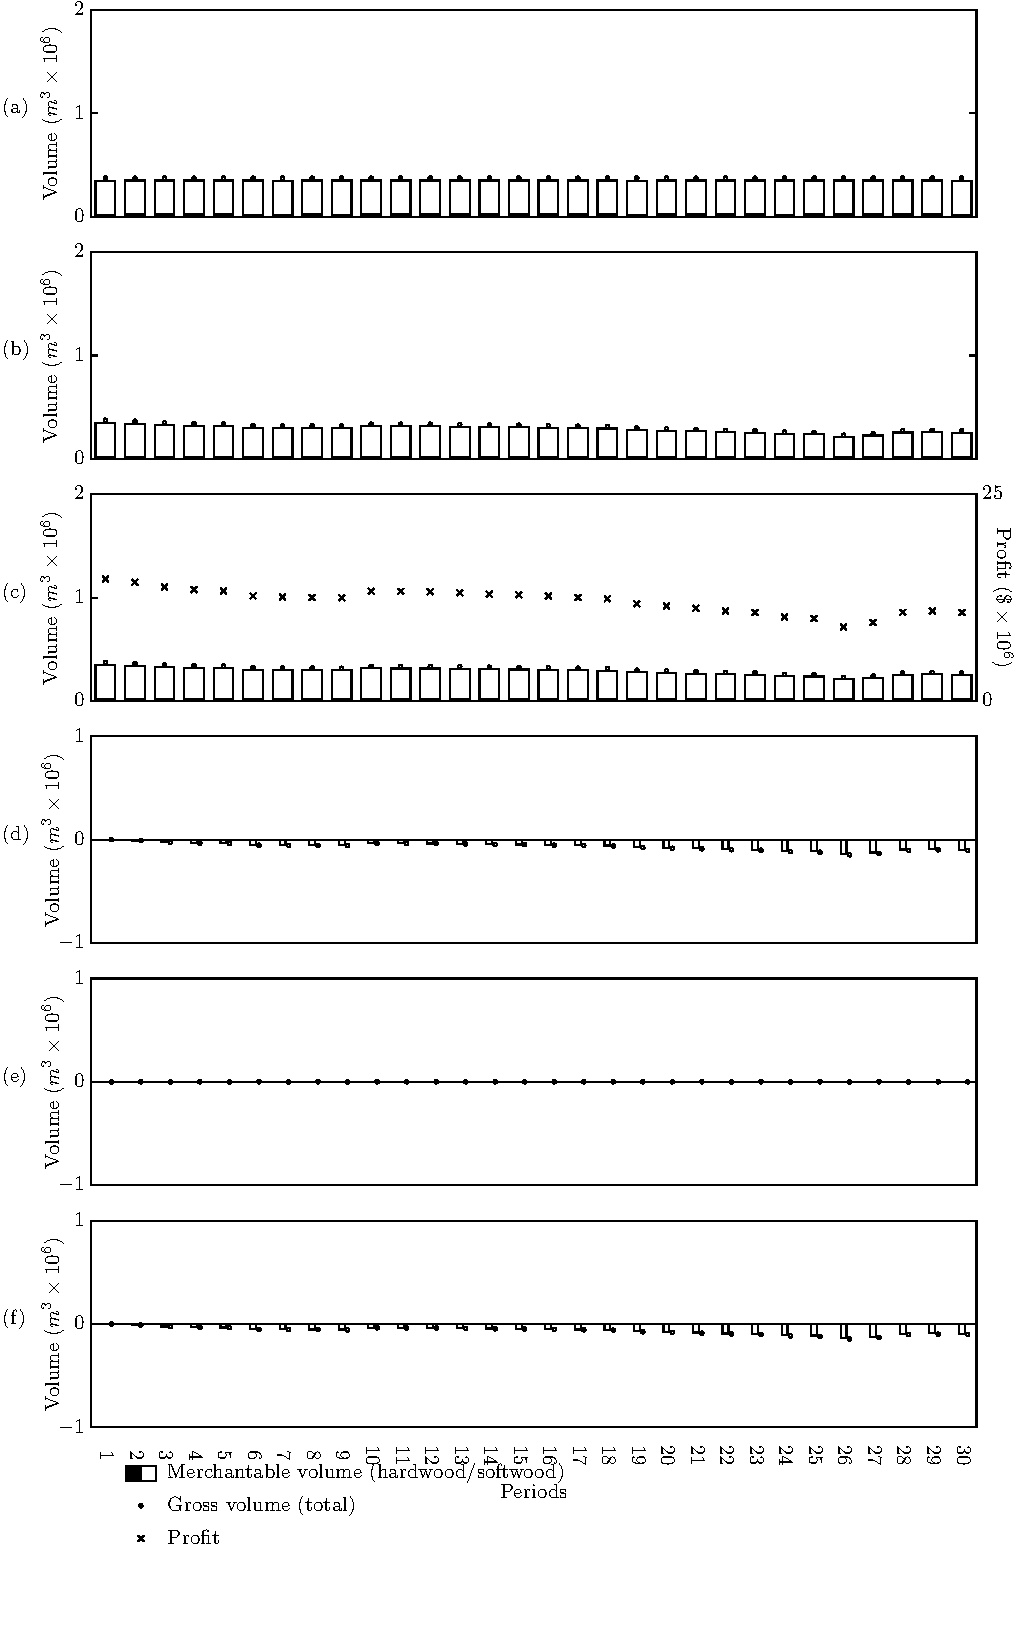
\includegraphics[width=10cm]{images/appendix/s6-5_hw000sw000}
  \caption{Scenario 6-5\_hw000sw000 (hardwood: 0\%, softwood: 0\%).}
  \label{fig:s6-5_hw000sw000}
\end{figure}

\begin{figure}[h]
  \centering
  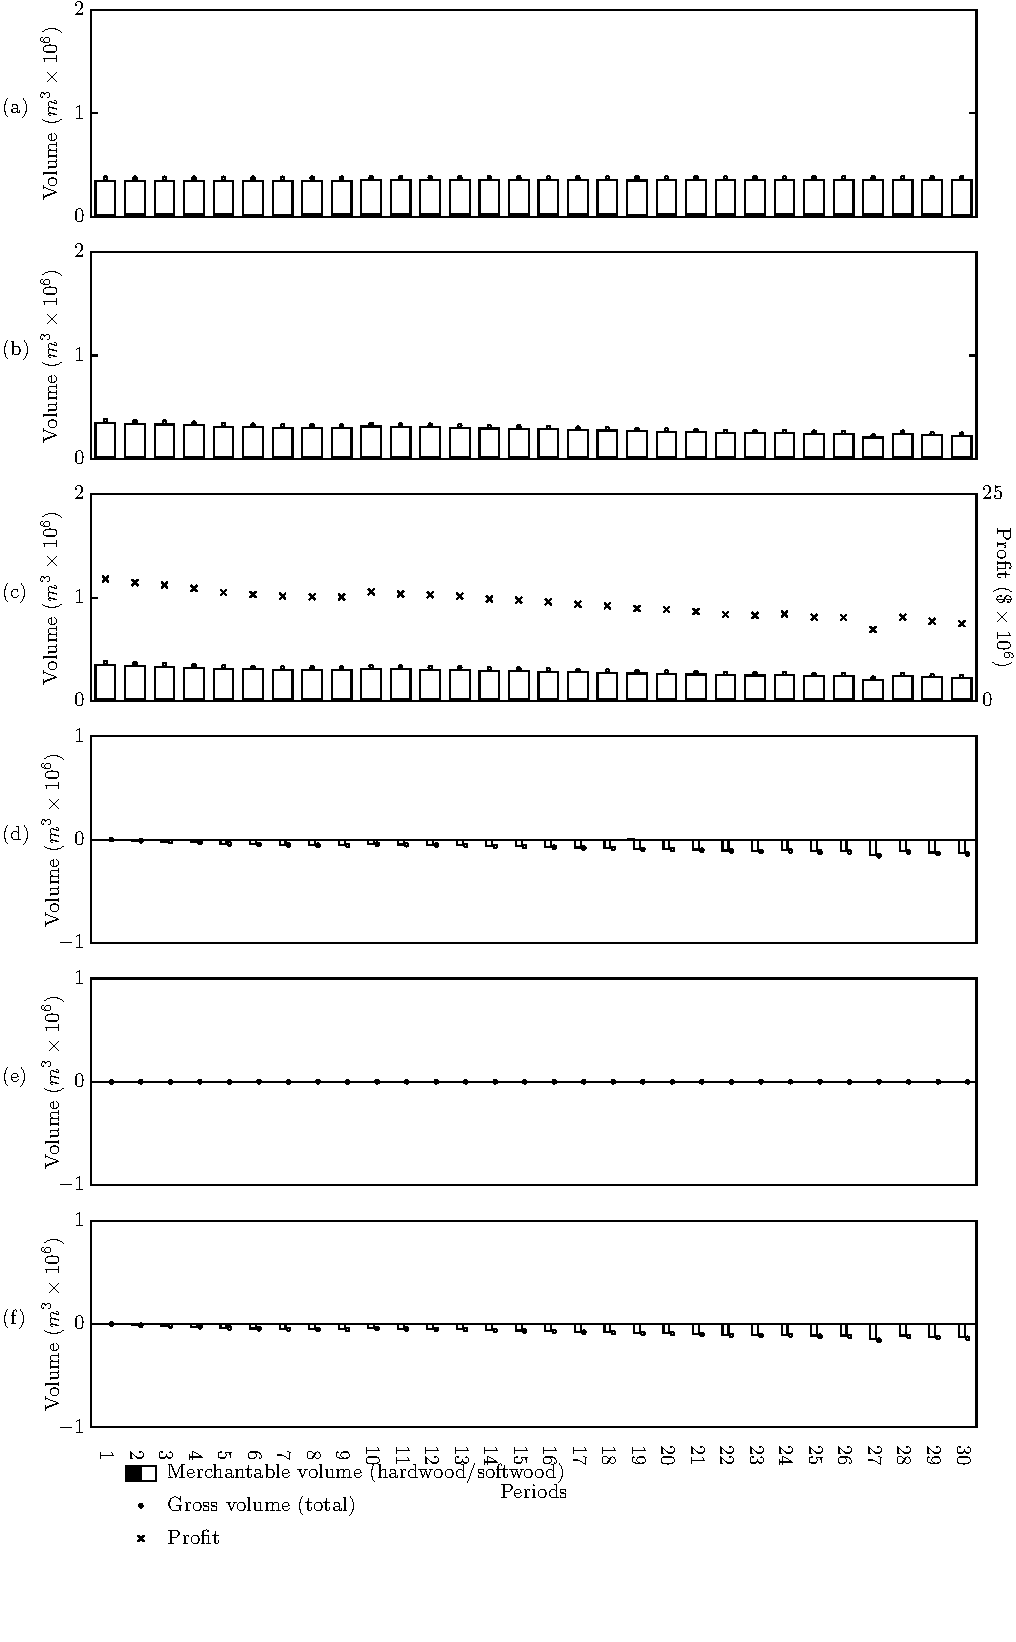
\includegraphics[width=10cm]{images/appendix/s6-5_hw001sw001}
  \caption{Scenario 6-5\_hw001sw001 (hardwood: 1\%, softwood: 1\%).}
  \label{fig:s6-5_hw001sw001}
\end{figure}

\begin{figure}[h]
  \centering
  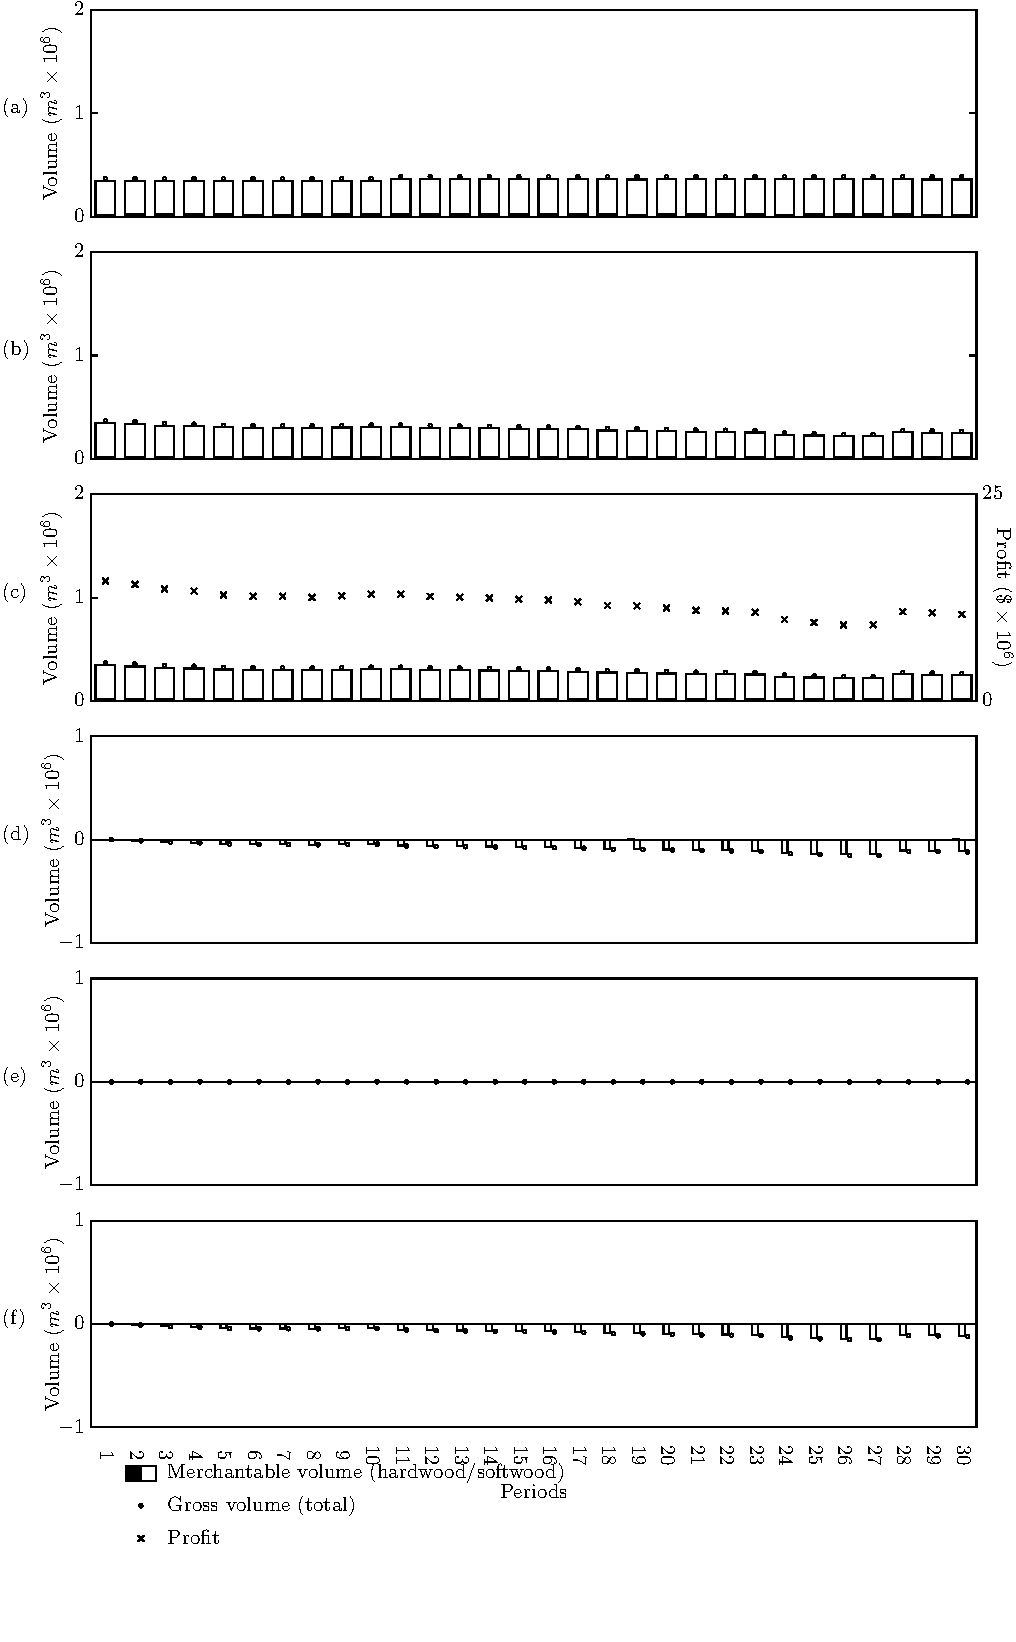
\includegraphics[width=10cm]{images/appendix/s6-1_p30a01}
  \caption{Scenario 6-5\_hw005sw005 (hardwood: 5\%, softwood: 5\%).}
  \label{fig:s6-5_hw005sw005}
\end{figure}


\begin{figure}[h]
  \centering
  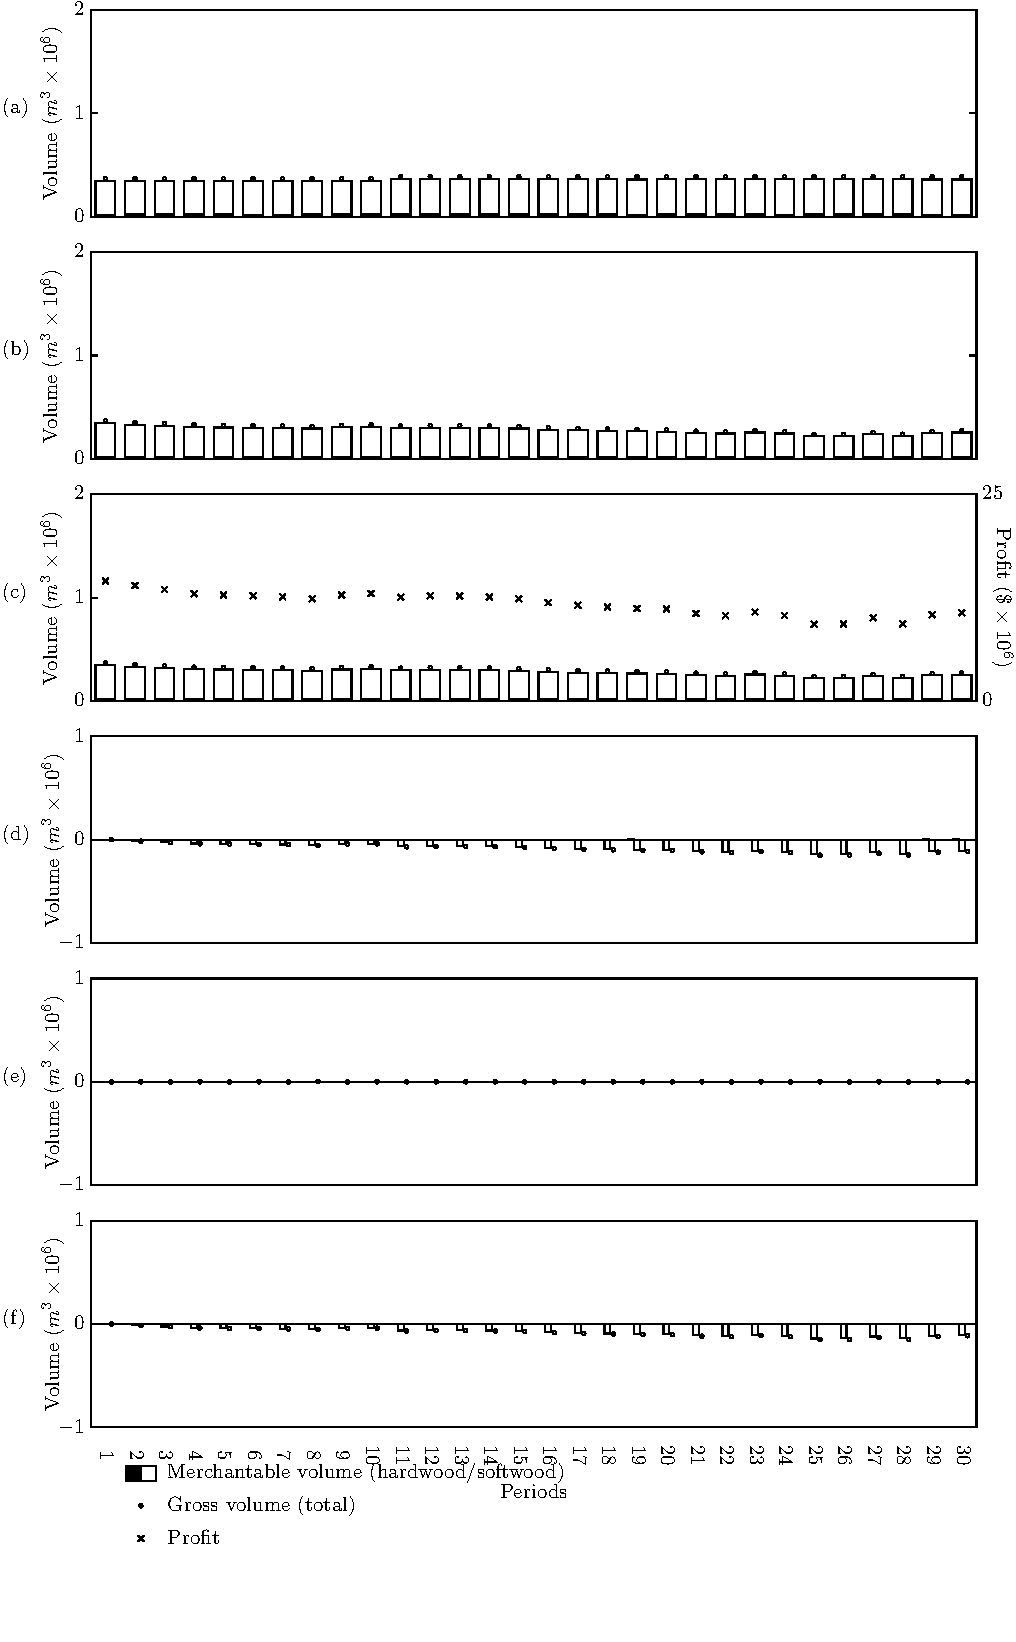
\includegraphics[width=10cm]{images/appendix/s6-5_hw099sw005}
  \caption{Scenario 6-5\_hw099sw005 (hardwood: 99\%, softwood: 5\%).}
  \label{fig:s6-5_hw099sw005}
\end{figure}

\begin{figure}[h]
  \centering
  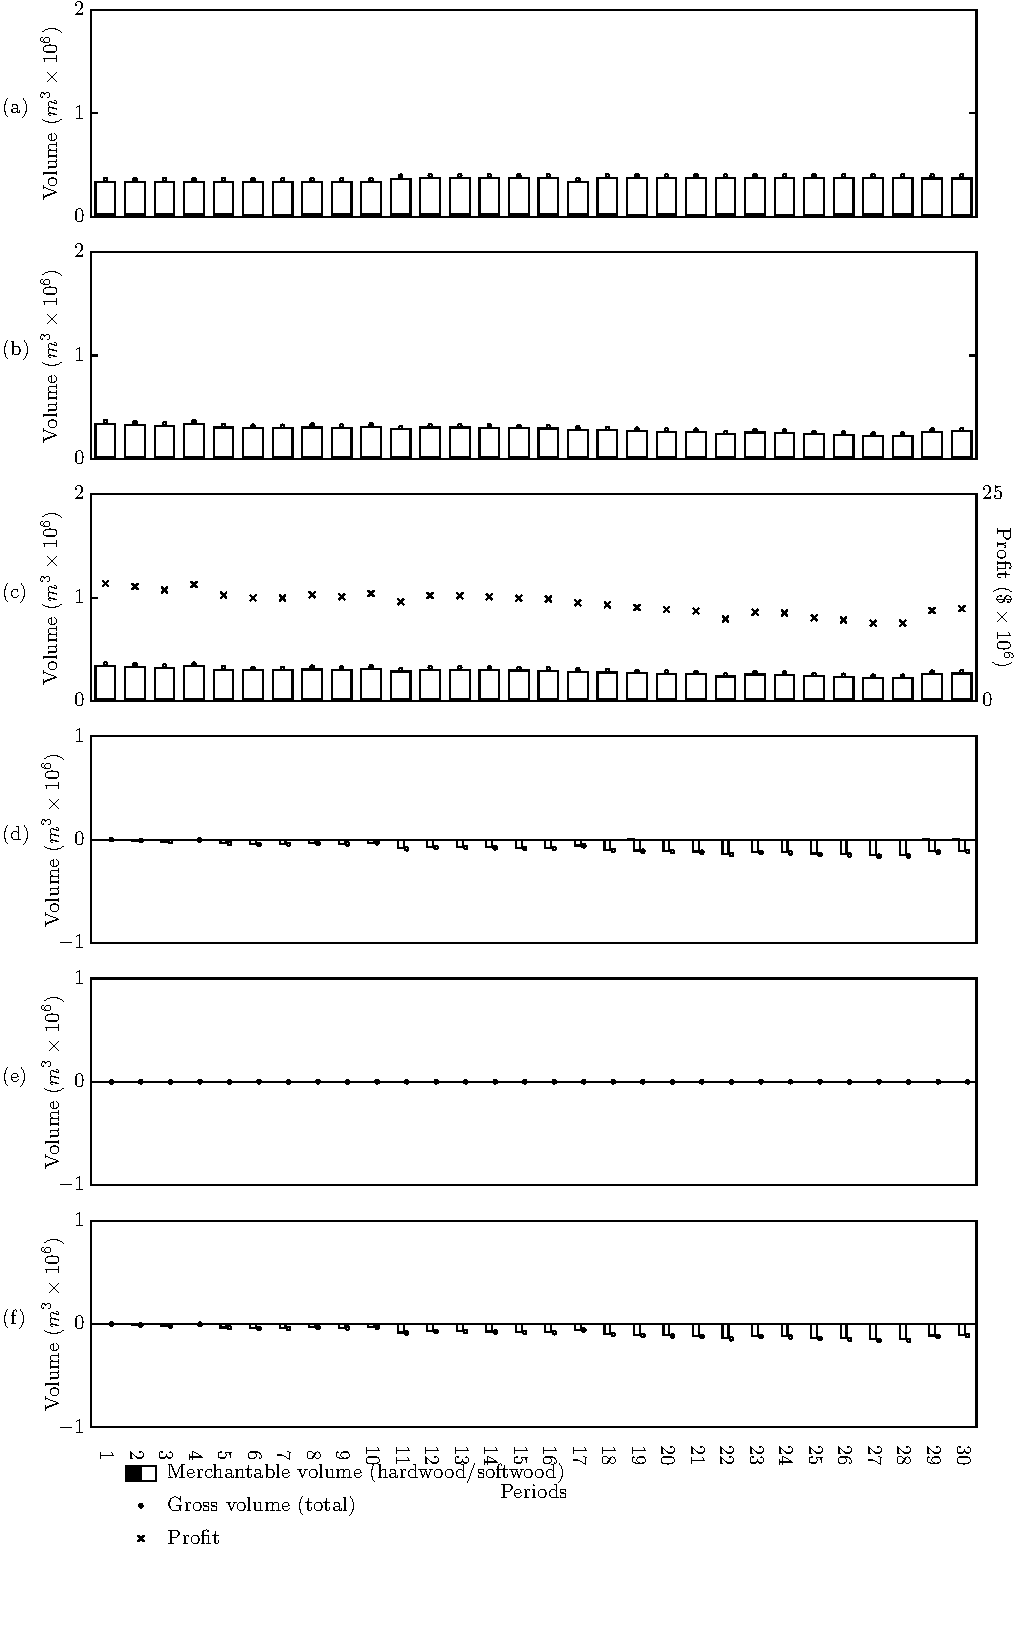
\includegraphics[width=10cm]{images/appendix/s6-5_hw010sw010}
  \caption{Scenario 6-5\_hw010sw010 (hardwood: 10\%, softwood: 10\%).}
  \label{fig:s6-5_hw010sw010}
\end{figure}

\begin{figure}[h]
  \centering
  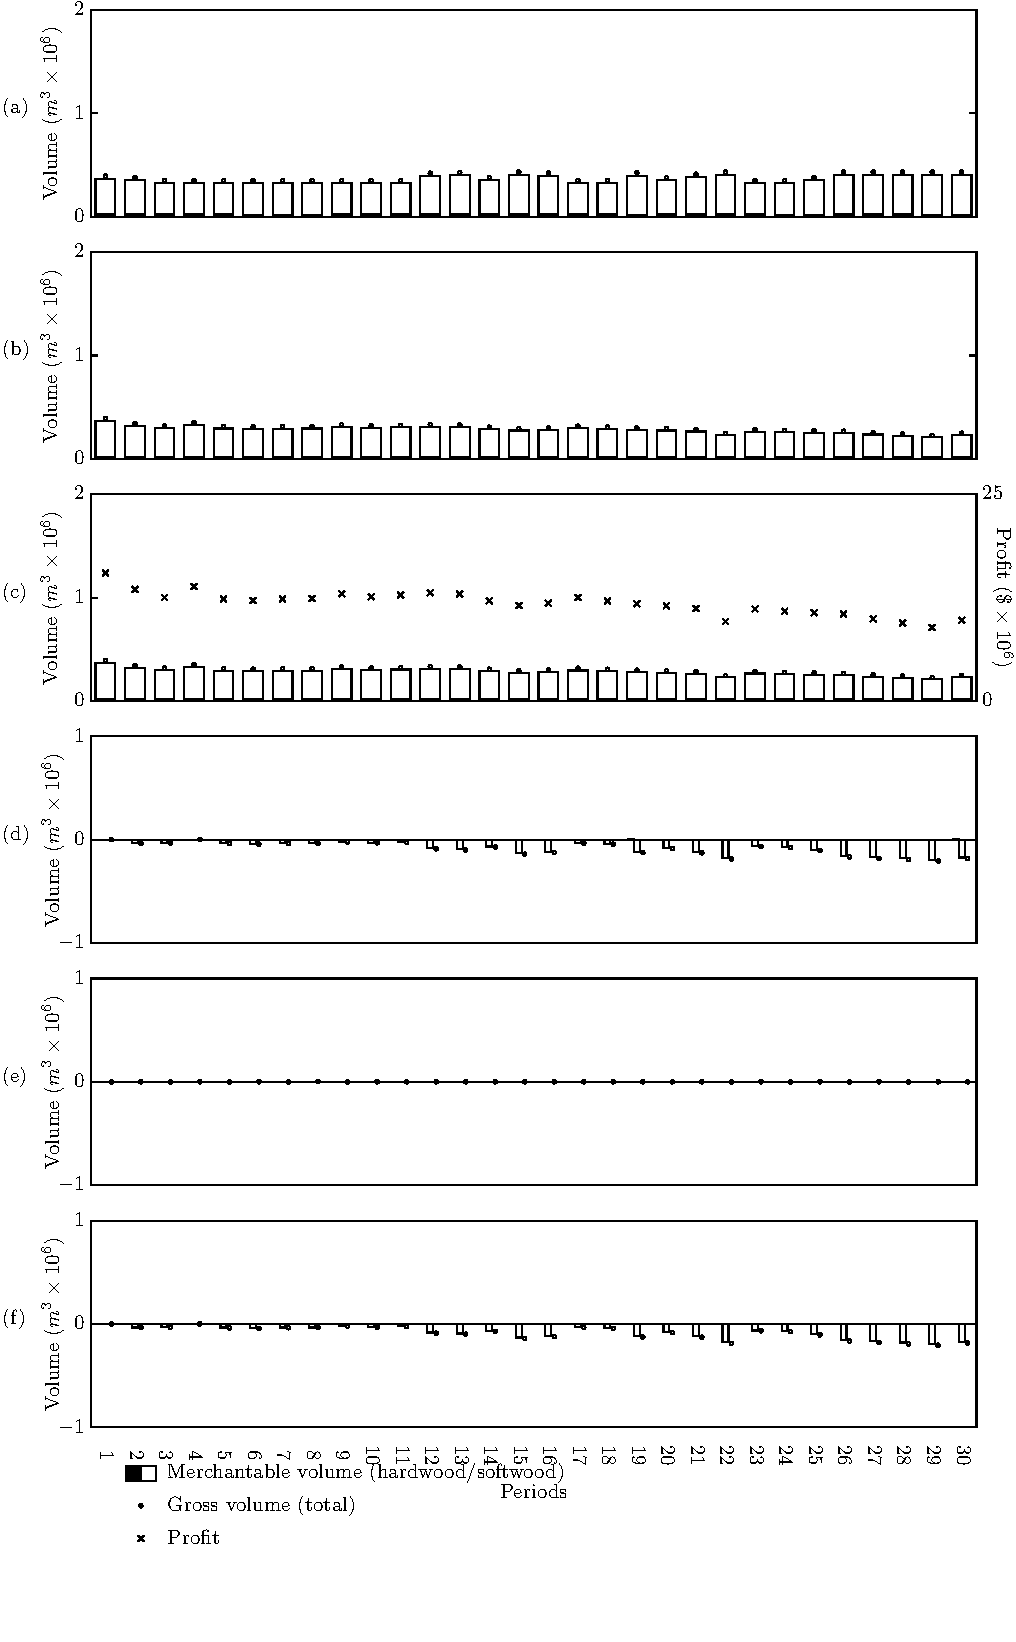
\includegraphics[width=10cm]{images/appendix/s6-5_hw020sw020}
  \caption{Scenario 6-5\_hw020sw020 (hardwood: 20\%, softwood: 20\%).}
  \label{fig:s6-5_hw020sw020}
\end{figure}

\begin{figure}[h]
  \centering
  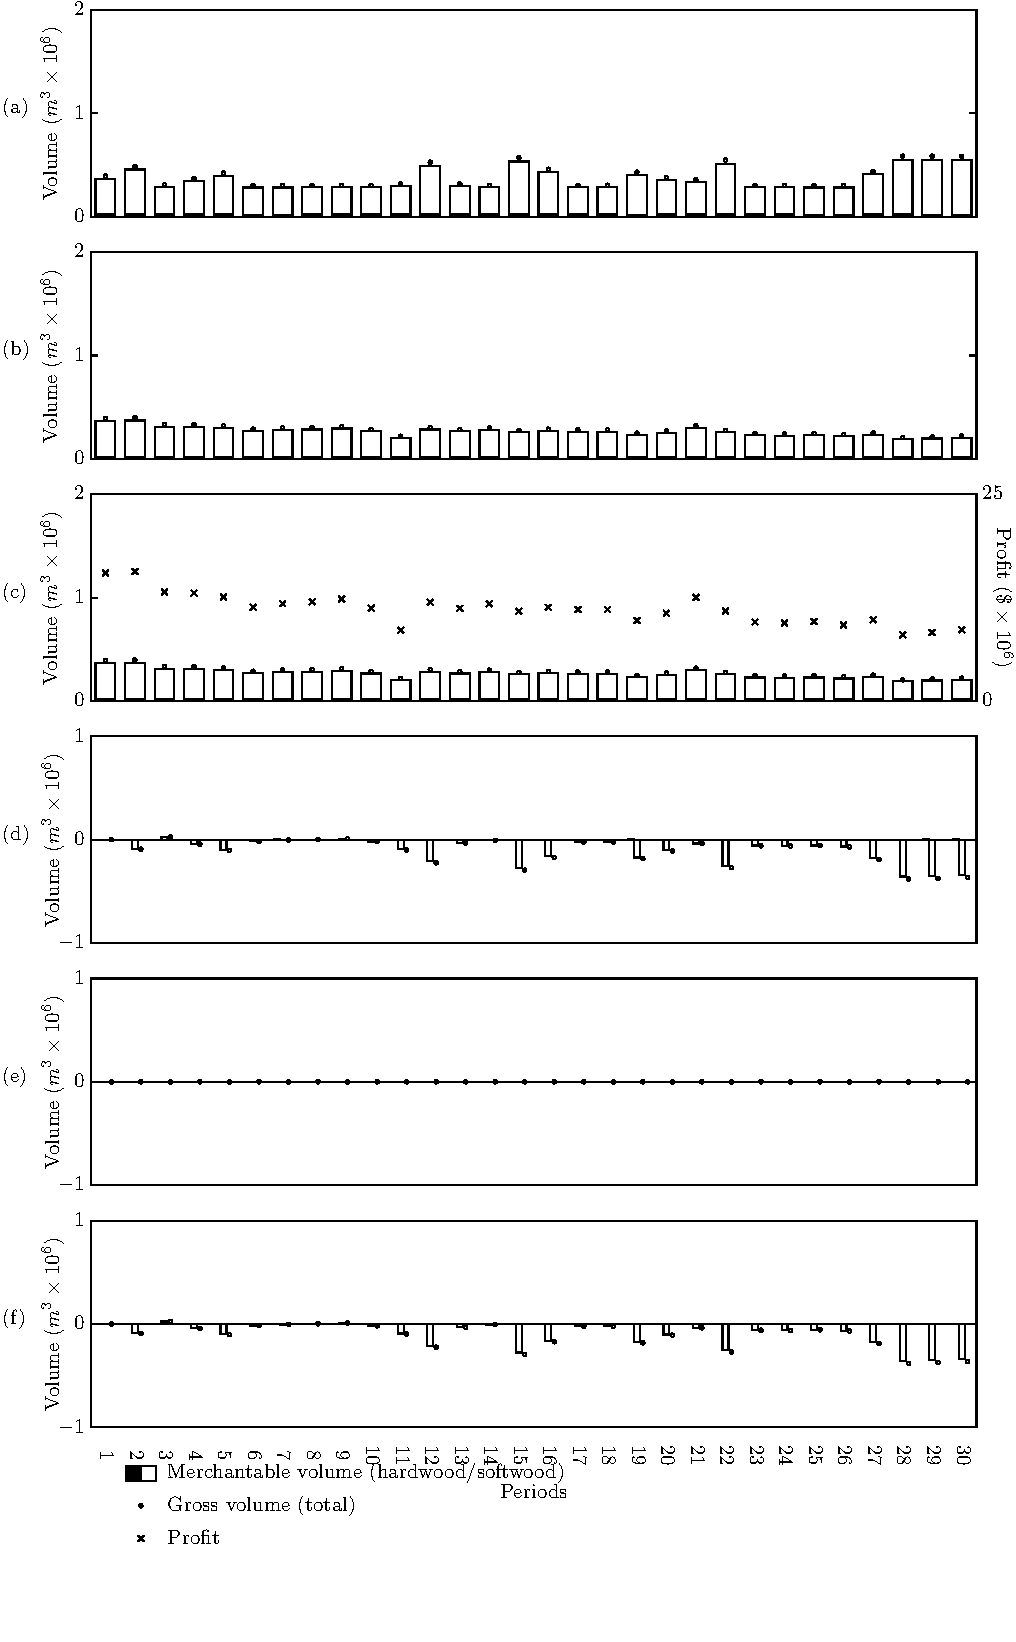
\includegraphics[width=10cm]{images/appendix/s6-5_hw050sw050}
  \caption{Scenario 6-5\_hw050sw050 (hardwood: 50\%, softwood: 50\%).}
  \label{fig:s6-5_hw050sw050}
\end{figure}
